\chapter{Approach}
\label{chap:approach}
There are four steps in the design and implementation of the portable probabilistic programming framework. At first we designed the syntax of the embedded programming language, which targets the description of the Bayesian networks and conditional query.  The design of the language is based on BUGS, but the syntax is more specific and efficient to be lightweight for the portable characteristic. Also the syntax can be expressive for most of the probabilistic models. The description of the models using the portable probabilistic programming language is separated from the code of the host language as well of the conditional query, which can enhance the reusability of the probabilistic models. The parser is implemented and the inference engine is generated automatically based on the conditional query. More details will be illustrated in section ~\ref{sec:syntax}. 

We implemented the probabilistic library for most of the probabilistic distribution such as Gaussian, Gama, Beta, etc. Our probabilistic programs define distributions by defining a distribution over possible execution traces. The distribution is fully specified by a generative procedure. More details can be found in section ~\ref{sec:distr}. 

The inference algorithm is based on the MCMC sampling, including rejection sampling and Metropolis-Hastings Algorithm, which is efficient and lightweight to implement. We will elaborate more on the mechanism of the inference engine through an example in section ~\ref{sec:infer}. 

Additionally, we implement the APIs for other languages leveraging some existing development tool such as SWIG (Simplified Wrapper and Interface Generator). More details for the APIs are in section ~\ref{sec:api}.

Our main contribution lies in the design of the portable probabilistic programming language to make it portable, the implementation of the probabilistic library and the lightweight implementation of the inference engine.


\section{Syntax of Programming Language}
\label{sec:syntax}
We will give some intuition of our portable probabilistic programming language by giving an example declaring the flip model, which is showed in Figure ~\ref{fig:flip_eg}. 

\begin{figure}
    \centering
    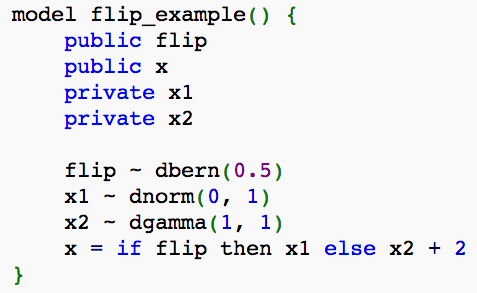
\includegraphics[width=0.6\textwidth]{figures/flip_eg.png}
    \caption{Flip example, describing the probabilistic model in our language.}
    \label{fig:flip_eg}
\end{figure}

The flip\_example describes a probabilistic model that has the distribution over variables as showed in Figure ~\ref{fig:flip_dist}. The grammar for this specific example is showed in Figure ~\ref{fig:flip_syn}. Under this syntax, the parser will parse the probabilistic program and generate the Bayesian network as the user described. The inference is done based on the probabilistic graph. The Bayesian network of the flip example is showed in Figure ~\ref{fig:flip_net}.


\begin{figure}
    \centering
    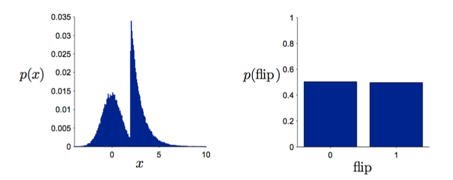
\includegraphics[width=0.9\textwidth]{figures/flip_dist.png}
    \caption{Flip example, the implied distributions over variables.}
    \label{fig:flip_dist}
\end{figure}

\begin{figure}
    \centering
    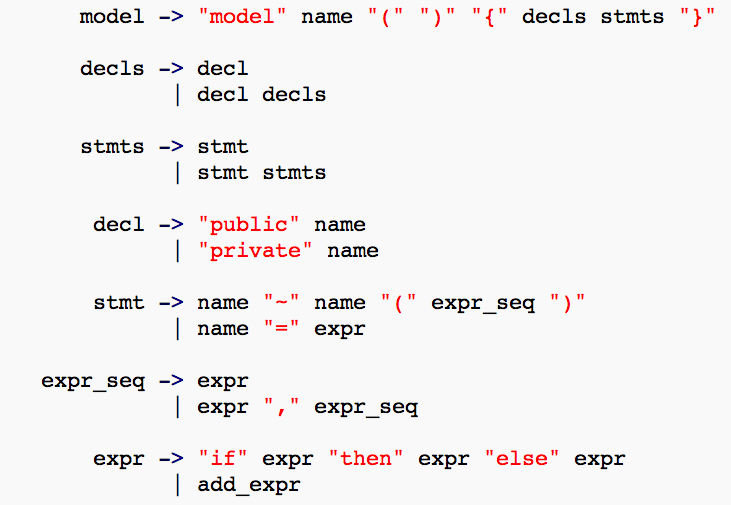
\includegraphics[width=0.7\textwidth]{figures/flip_syn.png}
    \caption{The grammar for the flip example.}
    \label{fig:flip_syn}
\end{figure}


\begin{figure}
    \centering
    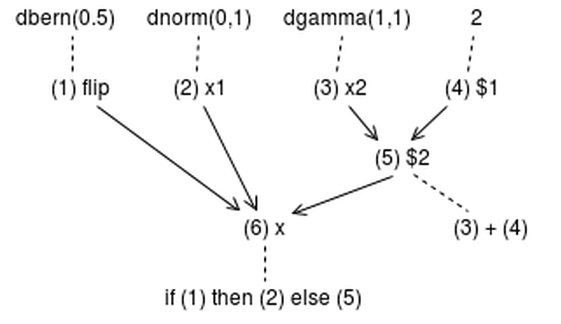
\includegraphics[width=0.6\textwidth]{figures/flip_net.png}
    \caption{The generated Bayesian network for the flip example.}
    \label{fig:flip_net}
\end{figure}

The grammar for the portable probabilistic programming language is as below:
\begin{align*}
           models \rightarrow & ~model \\
                   |& ~model ~models \\       
            model \rightarrow & ~\textcolor{red}{``model"} ~name \textcolor{red}{``("}~~~~~~~~~~~~~~~~~ \textcolor{red}{``)"} ~ \textcolor{red}{``\{"} decls ~stmts \textcolor{red}{``\}"} \\
                   |& ~\textcolor{red}{``model"} name \textcolor{red}{``("} model\_params \textcolor{red}{``)"} ~\textcolor{red}{``\{"} decls ~stmts \textcolor{red}{``\}"} \\         
     model\_params \rightarrow & ~name \\
                   |& ~name ~\textcolor{red}{``,"}~ model\_params \\        
            decls \rightarrow & ~decl \\
                   |& ~decl ~decls \\ 
            stmts \rightarrow & ~stmt \\
                   |& ~stmt ~stmts \\        
             decl \rightarrow & ~\textcolor{red}{``public"} ~variable \\
                   |& ~\textcolor{red}{``private"} ~variable \\         
             stmt \rightarrow & ~variable ~\textcolor{red}{``\sim"} ~name ~\textcolor{red}{``("} ~expr\_seq ~\textcolor{red}{``)"} \\
                   |& ~variable ~\textcolor{red}{``="} ~expr \\
                   |& ~\textcolor{red}{``for"} ~name ~\textcolor{red}{``="} ~expr ~\textcolor{red}{``to"} ~expr ~\textcolor{red}{``\{"} stmts \textcolor{red}{``\}"} \\        
         expr\_seq \rightarrow & ~expr \\
                   |& ~expr ~\textcolor{red}{``,"} ~expr\_seq \\      
             expr \rightarrow & ~\textcolor{red}{``if"} ~expr ~\textcolor{red}{``then"} ~expr ~\textcolor{red}{``else"} ~expr \\
                   |& ~\textcolor{red}{``new"} ~name ~\textcolor{red}{``("} ~\textcolor{red}{``)"} \\
                   |& ~add\_expr \\  
         add\_expr \rightarrow & ~term \\
                   |& ~term ~\textcolor{red}{``+"} ~add\_expr \\
                   |& ~term ~\textcolor{red}{``-"} ~add\_expr     
\end{align*}

\begin{align*}             
             term \rightarrow & ~primary \\  
                   |& ~primary \textcolor{red}{``*"} ~term \\
                   |& ~primary \textcolor{red}{``/"} ~term \\
          primary \rightarrow & ~numerical\_value \\
                   |& ~variable \\
                   |& ~function\_call \\
                   |& ~\textcolor{red}{``("} ~expr ~\textcolor{red}{``)"} \\
                   |& ~\textcolor{red}{``-"} ~primary \\           
    function\_call \rightarrow & ~name ~\textcolor{red}{``("} ~expr\_seq ~\textcolor{red}{``)"} \\           
         variable \rightarrow & ~name \\
                   |& ~field\_var \\
                   |& ~index\_var \\              
        field\_var \rightarrow & ~name ~\textcolor{red}{``."} ~name \\
        index\_var \rightarrow & ~name ~\textcolor{red}{``["} ~expr\_seq ~\textcolor{red}{``]"} \\           
  numerical\_value \rightarrow & ~integer\_value \\
                   |& ~integer\_value ~\textcolor{red}{``."} ~integer\_value \\                  
    integer\_value \rightarrow & ~[0-9]+ \\            
             name \rightarrow & ~[a-zA-Z\_][0-9a-zA-Z\_]*
\end{align*}

\section{Probabilistic Distribution Library}
\label{sec:distr}
We implemented the probabilistic library for most of the probabilistic distribution such as Gaussian, Gama, Beta, etc. Our probabilistic programs define distributions by defining a distribution over possible execution traces. The distribution is fully specified by a generative procedure. Some complex distributions are crafted compositionally. An example is showed on how to implement a Gaussian Mixture Model distribution in Figure ~\ref{fig:gmm}. As can be seen in Figure ~\ref{fig:gmm}., everytime we run the function gmm(), it will return a value based on the distribution implementation. And the trace of the returned value will meet the requirements of the density probability the program has defined.

\begin{figure}
    \centering
    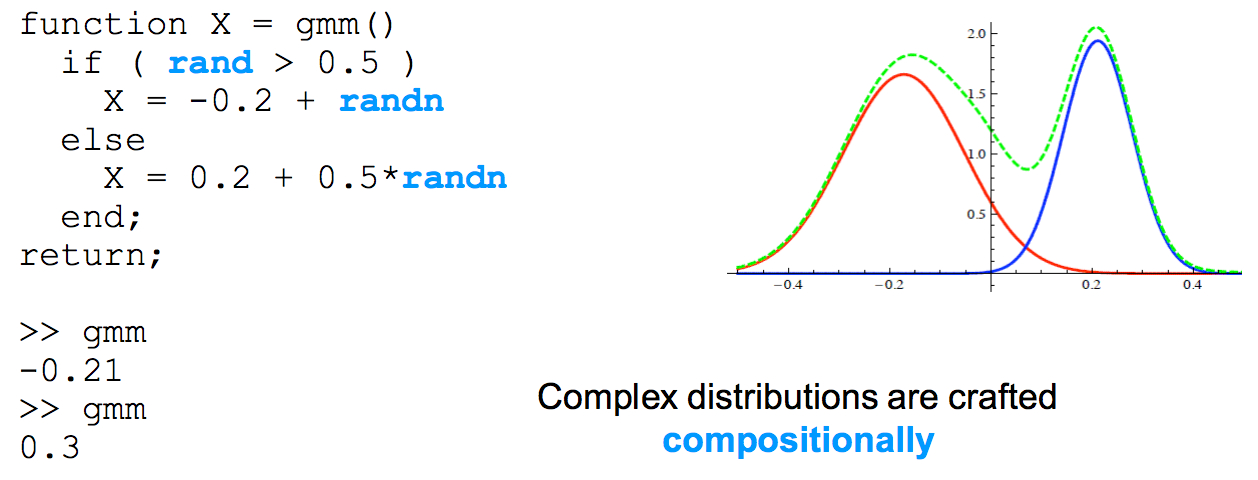
\includegraphics[width=0.9\textwidth]{figures/gmm.png}
    \caption{Implementation of GMM distribution example.}
    \label{fig:gmm}
\end{figure}


Most of the distributions in our library are implemented based on Normal distribution and Bernoulli distribution according to the mathematical methods. The probabilistic distributions in our library contain Bernoulli distribution, Normal distribution, Gamma distribution, Binomial distribution, Multinomial distribution, Dirichlet distribution, Beta distribution, Uniform distribution, and Poisson distribution.

\section{Inference Engine}
\label{sec:infer}
Calculating the distribution specified by a probabilistic program is called probabilistic inference. The inferred probability distribution is called the \textit{posterior probability distribution}, and the initial guess made by the program is called the \textit{prior probability distribution}. There are a number of methods for performing inference. The most common exact inference methods are: variable elimination, which eliminates (by integration or summation) the non-observed non-query variables one by one by distributing the sum over the product; clique tree propagation, which caches the computation so that many variables can be queried at one time and new evidence can be propagated quickly; and recursive conditioning and AND/OR search, which allow for a space-time tradeoff and match the efficiency of variable elimination when enough space is used. All of these methods have complexity that is exponential in the network's treewidth. The most common approximate inference algorithms are importance sampling, stochastic MCMC simulation ~\cite{mcmc}, mini-bucket elimination, loopy belief propagation, generalized belief propagation, and variational methods.

The mechanism of our inference engine is based on sampling. Currently we used Rejection Sampling algorithm in the inference engine, which is straightforward and easy to implement. However, rejection Sampling is not as efficient as other sampling algorithms like Gibbs Sampling and Metropolis-Hastings algorithm. Henceforth, we added another optional inference algorithm in our inference engine: Metropolis-Hastings algorithm. 

\subsection{Rejection Sampling}
\textit{Rejection sampling} is a basic technique used to generate observations from a distribution. It is a type of Monte Carlo method. The method works for any distribution in $\mathbb{R}^m$ with a density.

\begin{figure}
    \centering
    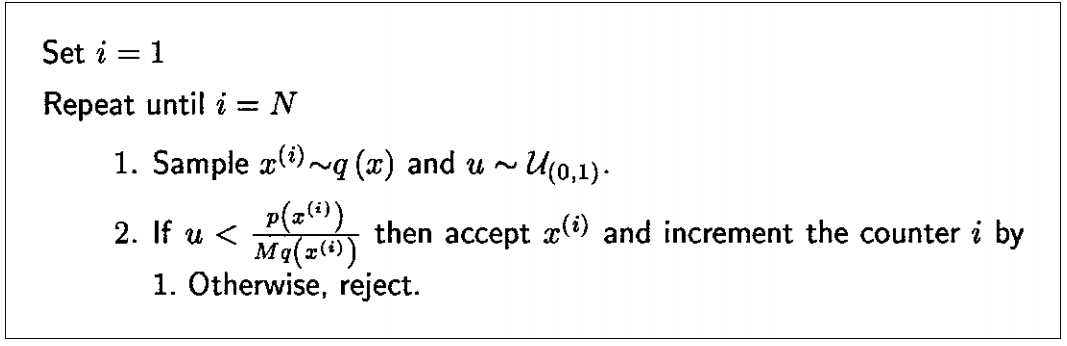
\includegraphics[width=0.9\textwidth]{figures/rj1.png}
    \caption{Rejection sampling algorithm. Here, $u \sim Uiform(0,1)$ denotes the operation of sampling a uniform random variable on the interval $(0,1)$.}
    \label{fig:rj1}
\end{figure}

\begin{figure}
    \centering
    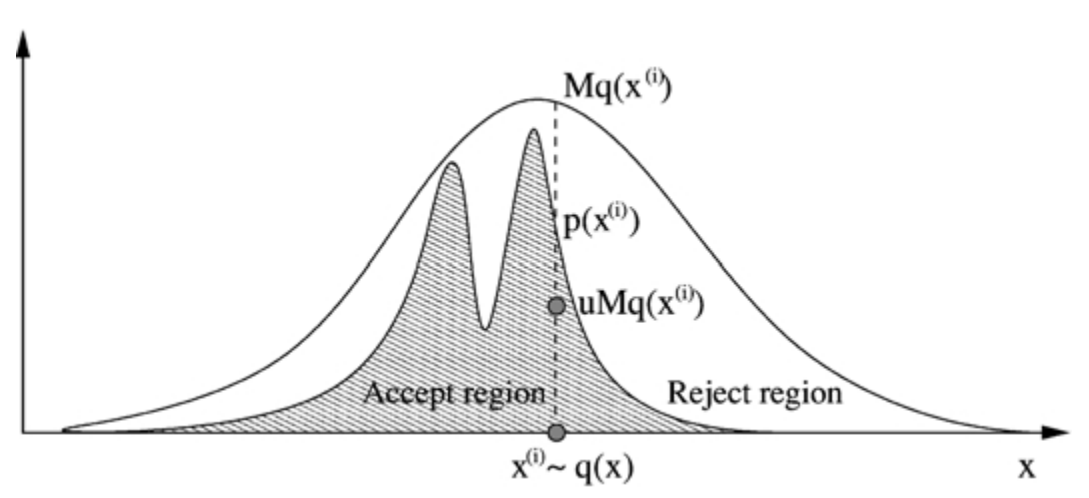
\includegraphics[width=0.7\textwidth]{figures/rj2.png}
    \caption{Rejection sampling: Sample a candidate $x(i)$ and a uniform variable $u$. Accept the candidate sample if $uMq(x^{(i)}) < p(x^{(i)})$, otherwise reject it.}
    \label{fig:rj2}
\end{figure}

Rejection sampling is based on the observation that to sample a random variable one can sample uniformly from the region under the graph of its density function. We can sample from a distribution $p(x)$, which is known up to a proportionality constant, by sampling from another easy-to-sample proposal distribution $q(x)$ that satisfies $p(x) \leq Mq(x), M < \infty$, using the accept/reject procedure describe in Figure ~\ref{fig:rj1} (see also Figure ~\ref{fig:rj2}). ~\cite{mcmc}
The accepted $x(i)$ can be easily shown to be sampled with probability $p(x)$ ~\cite{robert}. This simple method suffers from severe limitations. It is not always
possible to bound $p(x) \/ q(x)$ with a reasonable constant M over the whole space $X$. If $M$ is too large, the acceptance probability 
\begin{align*}
  Pr(x ~ accepted) = Pr(u < \frac{p(x)}{Mq(x)}) = \frac{1}{M}
\end{align*}
will be too small. This makes the method impractical in high-dimensional scenarios.

Continue with our previous e
\subsection{Metropolis-Hastings Algorithm}

\begin{figure}
    \centering
    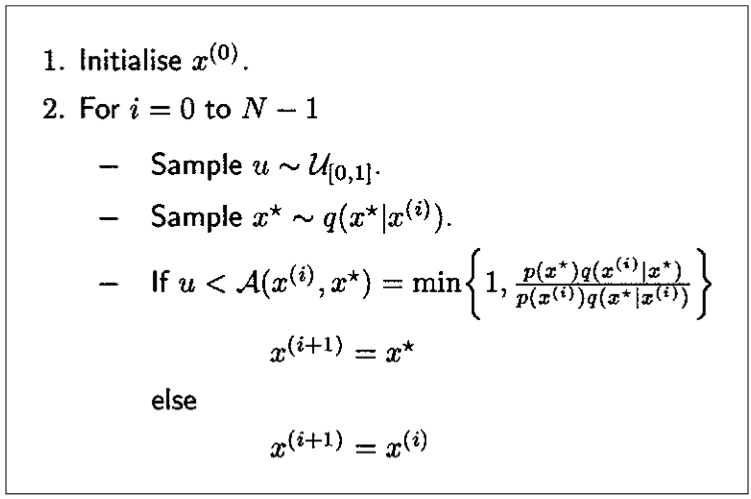
\includegraphics[width=0.7\textwidth]{figures/mh.png}
    \caption{Metropolis-Hastings algorithm.}
    \label{fig:mh}
\end{figure}

\begin{figure}
    \centering
    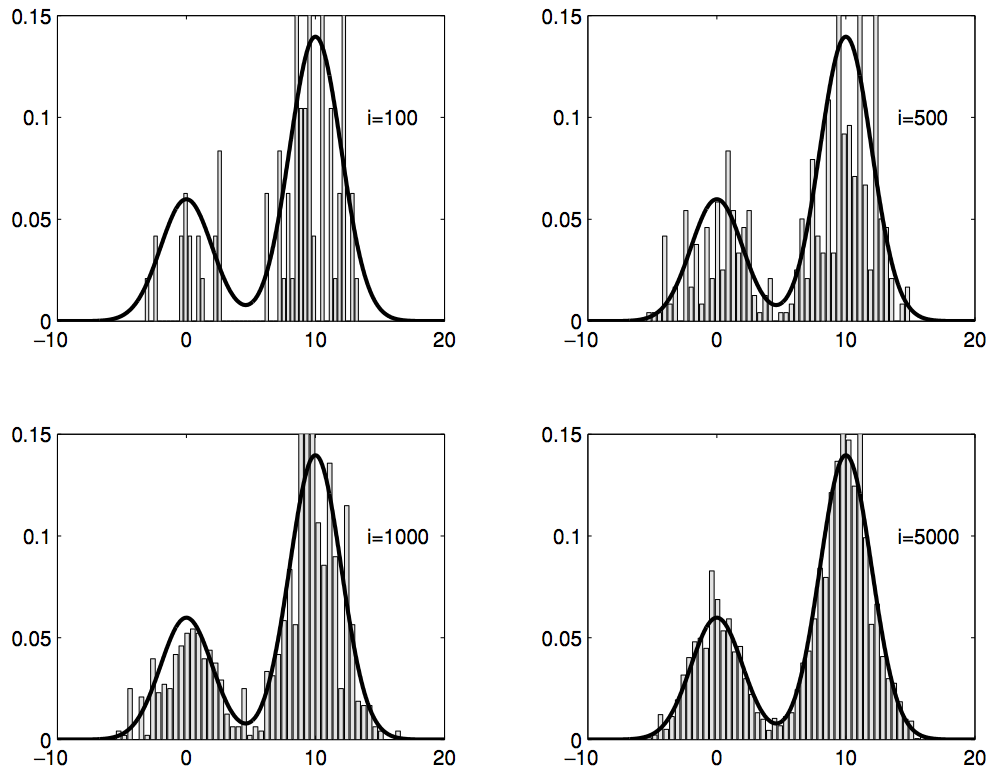
\includegraphics[width=0.7\textwidth]{figures/mh2.png}
    \caption{Target distribution and histogram of the MCMC samples at different iteration points.}
    \label{fig:mh2}
\end{figure}


The \textit{Metropolis-Hastings (MH) algorithm} is the most popular MCMC method. An MH step of invariant distribution $p(x)$ and proposal distribution $q(x^*	| x)$ involves sampling a candidate value $x^*$ given the current value $x$ according to $q(x^* | x)$. The Markov chain then moves towards $x^*$ with acceptance probability
\begin{align*}
  A(x, x^*) = min\{1,[p(x)q(x^* | x)]^{−1} p(x^*)q(x | x^*)\}
\end{align*}
otherwise it remains at $x$. The pseudo-code is shown in Figure ~\ref{fig:mh}, while Figure ~\ref{fig:mh2} shows the results of running the MH algorithm with a Gaussian proposal distribution
\begin{align*}
  q(x^* | x(i)) = Normal(x^{(i)}, 100)
\end{align*}
and a bimodal target distribution
\begin{align*}
  p(x) \propto 0.3 \times exp(−0.2x^2) + 0.7 exp(−0.2{(x - 10)}^2)
\end{align*}
for 5000 iterations. As expected, the histogram of the samples approximates the target distribution.

The MH algorithm is very simple, but it requires careful design of the proposal distribution $q(x^* | x)$. In subsequent sections, we will see that many MCMC algorithms arise by considering specific choices of this distribution. In general, it is possible to use suboptimal inference and learning algorithms to generate data-driven proposal distributions.
The transition kernel for the MH algorithm is
\begin{align*}
  K_{MH}(x^{(i + 1)} | x^{(i)}) = q(x^{(i + 1)} | x^{(i)}) \mathscr{A}(x^{(i)}, x^{(i + 1)}) + \sigma_{x^{(i)}} (x^{(i + 1)}) r (x^{(i)}),
\end{align*}  
where $r(x(i))$ is the term associated with rejection
\begin{align*}
  r(x^{(i)} = \int_{\chi} q(x^* | x^{(i)})(1 - \mathscr{A}(x^{(i)}), x^*))dx^*
\end{align*}
It is fairly easy to prove that the samples generated by MH algorithm will mimic samples
drawn from the target distribution asymptotically. By construction, $K_{MH}$ satisfies the detailed
balance condition
\begin{align*}
  p(x^{(i)})K_{MH}(x^{(i + 1)} | x^{(i)}) = p(x^{(i + 1)})K_{MH}(x^{(i)} | x^{(i + 1)})
\end{align*}
and, consequently, the MH algorithm admits $p(x)$ as invariant distribution. To show that the MH algorithm converges, we need to ensure that there are no cycles (aperiodicity)
and that every state that has positive probability can be reached in a finite number of steps (irreducibility). Since the algorithm always allows for rejection, it follows that it is aperiodic. To ensure irreducibility, we simply need to make sure that the support of $q(\cdotp)$ includes the support of $p(\cdotp)$.

The independent sampler and the Metropolis algorithm are two simple instances of the MH algorithm. In the independent sampler the proposal is independent of the current state, $q(x^* | x^{(i)}) = q(x^*)$. Hence, the acceptance probability is
\begin{align*}
  \mathscr{A}(x^{(i)} | x^*) = min \{1, \frac{p(x^*)q(x^{(i)})}{p(x^{(i)})q(x^*)}\}
\end{align*}
The Metropolis algorithm assumes a symmetric random walk proposal $q(x^* | x^{(i)}) = q(x^{(i)} | x^*)$ and, hence, the acceptance ratio simplifies to
\begin{align*}
  \mathscr{A}(x^{(i)}, x^*) = min \{ 1, \frac{p(x^*)}{p(x^{(i)})} \}
\end{align*}

\begin{figure}
    \centering
    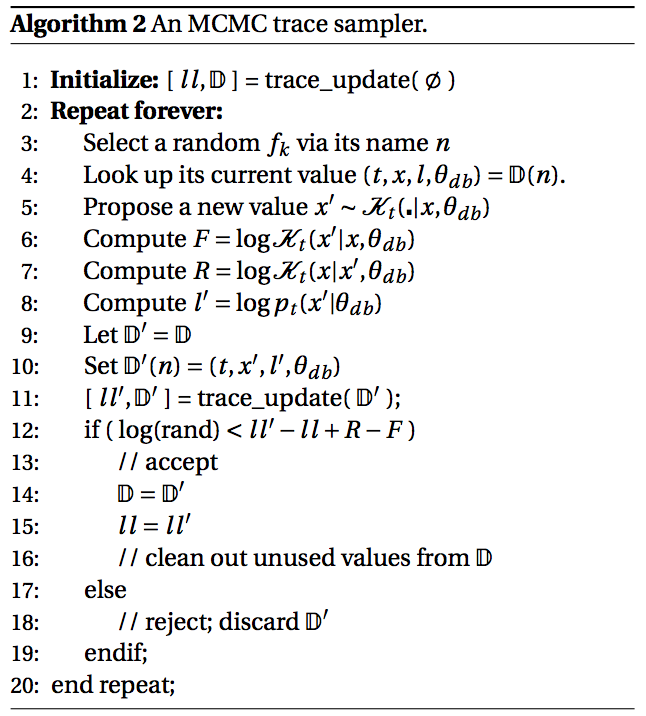
\includegraphics[width=0.7\textwidth]{figures/trace1.png}
    \caption{An MCMC trace sampler.}
    \label{fig:trace1}
\end{figure}

\begin{figure}
    \centering
    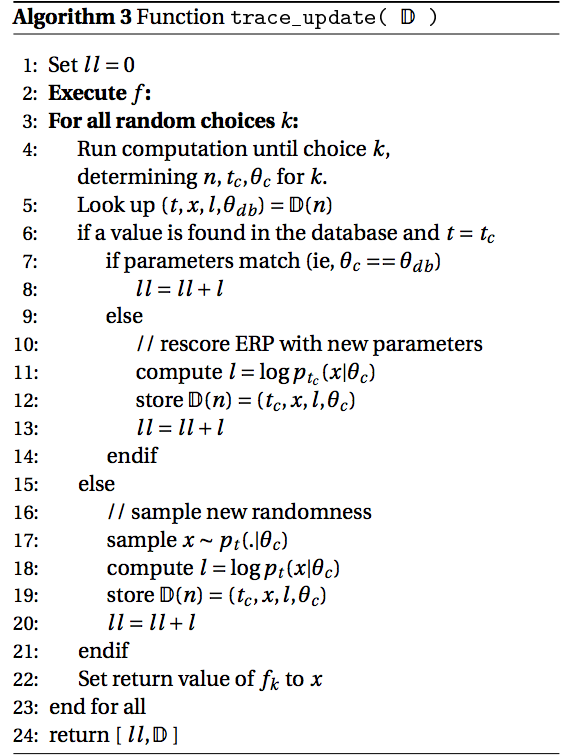
\includegraphics[width=0.7\textwidth]{figures/trace2.png}
    \caption{Algorithm for trace\_update}
    \label{fig:trace2}
\end{figure}

In the implementation of the MH alorithm in our inference engine, we leverage the approach proposed by ~\cite{lightweight}, which memorized trace information and update trace iteratively as illustrated in Figure ~\ref{fig:trace1} and Figure ~\ref{fig:trace2}. 

\subsection{Caculating the probability}
The intuitive idea is to sample the traces as the program runs. If the trace meets the Boolean requirements of the condition, then record the trace, or the trace is discarded. Then we calculate the number of the traces that can meet the Boolean requirement of the probability we want to get. Then calculating this number over the whole number of traces we recorded can derive the final conditional probability.

\section{APIs for Other Languages}
\label{sec:api}
We leverage the development tool SWIG (Simplified Wrapper and Interface Generator) ~\cite{swig} to make other languages be able to call for C functions, as we implemented in C. Once the user has the APIs, he/she is able to call the load probabilistic model function and inference function in each common language. That's how the portable is implemented. 

	The challenge in this part is the C/C++ pointer doesn’t exist in other languages like Java and Python. We cope with this problem by using wrapper with a specific form to hint the difference of the pointers and the normal variables.
  
  We will give some examples of how our framework can be used in other common language like \textbf{C, Python, Java}.
  
\subsection{C}

\subsection{Python}

\subsection{Java}

